\subsection{Zasada prawej ręki}

\subsection{Sprawdzenie przecinania się dwóch odcinków}
Przypuśćmy, że dysponujemy przestrzenią $\mathbb{R}^3$ oraz odcinkami danymi przez pary punktów 
$(P_1, P_2)$ oraz $(P_3, P_4)$. Naszym celem będzie sprawdzenie,
czy istnieje punkt wspólny pomiędzy tymi odcinkami.

Na początku omówmy geometryczną interpretację iloczynów skalarnych, którą wykorzystamy w dalszych rozważaniach.

Dane są wektory $\vec{u},\vec{v} \in \mathbb{R}^2$ oraz prosta $L$ prostopadła
do $\vec{u}$ przechodząca przez punkt $(0,0)$. Wtedy iloczyn skalarny 
standardowy $\vec{u} \cdot \vec{v}$
jest:
\begin{itemize}[]
	\item dodatni, jeśli groty $\vec{u}$ oraz $\vec{v}$ są po tej samej stronie płaszczyzny podzielonej przez prostą $L$,
	\item ujemny, jeśli groty $\vec{u}$ oraz $\vec{v}$ są po  przeciwnych stronach płaszczyzny podzielonej przez prostą $L$,
	\item zerowy w przypadku kiedy wektor $\vec{v}$
	leży na prostej $L$.
\end{itemize}

Teraz możemy sformułować uogólnienie zasady prawej ręki.
Dane są wektory $\vec{u},\vec{v},\vec{w} \in \mathbb{R}^3$.
Wtedy jeśli $(\vec{u} \times \vec{v})
\cdot (\vec{u} \times \vec{w}) > 0$, to bazy
$(\vec{u}, \vec{v},  (\vec{u} \times \vec{v}))$ oraz
$(\vec{u}, \vec{w},  (\vec{u} \times \vec{w}))$ są zgodne,
co interpretujemy geometrycznie jako sytuację, w której 
groty wektorów 
$\vec{v}, \vec{w}$ są po tej samej stronie względem prostej,
na której leży wektor $\vec{u}$.


Pomysł na algorytm polega na sprawdzeniu, czy punkty $P_1$
oraz $P_2$ znajdują po przeciwnych stronach prostej 
przechodzącej przez punkty $P_3$ i $P_4$ oraz 
na sprawdzeniu, czy punkty $P_3$
oraz $P_4$ znajdują się po przeciwnych stronach prostej 
przechodzącej przez punkty $P_1$ i $P_2$. Jeśli odpowiedź
na tak postawione pytanie jest twierdząca, to zadane
odcinki muszą się przecinać.


\begin{algorithm}[H]
	\caption{Sprawdzenie, czy dwa odcinki się przecinają w przestrzeni $\mathbb{R}^3$}
	\begin{algorithmic}[1]
		\Procedure{SegmentIntersectionR3}{($P_1, P_2$), ($P_3, P_4$): odcinki}
		\If{$P_1 = P_3 \lor P_1 = P_4 \lor P_2 = P_3 \lor P_2 = P_4$}
		\State \Return \true
		\EndIf
		\State $\vec{v}_{12} \gets P_2 - P_1$
		\State $\vec{v}_{34} \gets P_4 - P_3$
		\State $\vec{w} \gets \vec{v}_{12} \times \vec{v}_{34}$	
		\If{$\vec{w} = \mathbf{0}$} \Comment Jeśli odcinki są współliniowe
		\State $d \gets \max\{|P_1P_3|, |P_1P_4|, |P_2P_3|, |P_2P_4|\}$
		\If{$d \leq |P_1P_2| + |P_3P_4|$}
		\State \Return \true
		\EndIf
		\EndIf
		\State $\vec{v}_{13} \gets P_3 - P_1$
		\State $\vec{v}_{14} \gets P_4 - P_1$
		\If{$(\vec{v}_{12} \times \vec{v}_{14}) \cdot \vec{w}$ oraz 
		$(\vec{v}_{12} \times \vec{v}_{13}) \cdot \vec{w}$ są tego samego znaku}
		\State \Return \false
		\EndIf
		\State $\vec{v}_{32} \gets P_2 - P_3$
		\State $\vec{v}_{31} \gets P_1 - P_3$
		\If{$(\vec{v}_{34} \times \vec{v}_{31}) \cdot \vec{w}$ oraz 
		$(\vec{v}_{34} \times \vec{v}_{32}) \cdot \vec{w}$ są tego samego znaku}
		\State \Return \false
		\EndIf
		\State \Return \true
		\EndProcedure
	\end{algorithmic}
	\label{segment_intersection_r3}
\end{algorithm}

Zauważmy, że gdybyśmy powyższy problem rozwiązywali w przestrzeni $\mathbb{R}^2$,
to podczas badania iloczynów wektorowych jedyne co interesowałoby nas,
to znak trzeciej współrzędnej. Z zasady prawej ręki, jeśli
trzecia współrzędna wektora 
$\vec{u} \times \vec{v}$ jest dodatnia, to wektor $\vec{v}$
znajduje się po lewej stronie wektora $\vec{u}$ oraz jeśli 
jest ujemna, to wektor $\vec{v}$
znajduje się po prawej stronie wektora $\vec{u}$. 

Fakt ten znacznie upraszcza sprawdzanie orientacji wektorów iloczynem wektorowym.

Trzecią współrzędną iloczynu wektorowego $\vec{u} \times \vec{v}$ w $\mathbb{R}^2$
obliczymy korzystając ze wzoru:
\[c = \vec{u}_x \vec{v}_y - \vec{v}_x \vec{u}_y.\]



\begin{algorithm}[H]
	\caption{Sprawdzenie przecinania się dwóch odcinków w przestrzeni $\mathbb{R}^2$}
	\begin{algorithmic}[1]
		\Procedure{Prod2}{$\vec{u}$,$\vec{v}$: wektory}
		\State \Return $\vec{u}_x \vec{v}_y - \vec{v}_x \vec{u}_y$
		\EndProcedure
		\Procedure{SegmentIntersectionR2}{($P_1, P_2$), ($P_3, P_4$): odcinki}
		\If{$P_1 = P_3 \lor P_1 = P_4 \lor P_2 = P_3 \lor P_2 = P_4$}
		\State \Return \true
		\EndIf
		\State $\vec{v}_{12} \gets P_2 - P_1$
		\State $\vec{v}_{34} \gets P_4 - P_3$
		\If{\textsc{Prod2}$(\vec{v}_{12}$, $\vec{v}_{34}) = 0$} \Comment Jeśli odcinki są współliniowe
		\State $d \gets \max\{|P_1P_3|, |P_1P_4|, |P_2P_3|, |P_2P_4|\}$
		\If{$d \leq |P_1P_2| + |P_3P_4|$}
		\State \Return \true
		\EndIf
		\EndIf
		\State $\vec{v}_{13} \gets P_3 - P_1$
		\State $\vec{v}_{14} \gets P_4 - P_1$
		\If{$\textsc{Prod2}(\vec{v}_{12}$, $\vec{v}_{14})$ $\cdot$ $\textsc{Prod2}(\vec{v}_{12}$, $\vec{v}_{13}) > 0$}
		\State \Return \false
		\EndIf
		\State $\vec{v}_{32} \gets P_2 - P_3$
		\State $\vec{v}_{31} \gets P_1 - P_3$
		\If{$\textsc{Prod2}(\vec{v}_{34}$, $\vec{v}_{31})$ $\cdot$ $\textsc{Prod2}(\vec{v}_{34}$, $\vec{v}_{32}) > 0$}
		\State \Return \false
		\EndIf
		\State \Return \true
		\EndProcedure
	\end{algorithmic}
	\label{segment_intersection_r2}
\end{algorithm}


\subsection{Problem przynależności punktu do wielokąta}


\subsection{Metoda zamiatania}
\subsubsection{Znajdowanie długości sumy odcinków}
Mamy zbiór być może nakładających się odcinków w jednowymiarowej przestrzeni euklidesowej, które siłą rzeczy
znajdują się na jednej prostej. Naszym zadaniem jest policzyć długość tych odcinków, ale w taki sposób, że każdy
fragment przestrzeni należy do więcej niż jednego odcinka liczymy tylko raz (czyli obliczamy pole sumy
teoriomnogościowej tych odcinków).

Aby rozwiązać ten problem, skorzystamy z metody zamiatania. Dla
uproszczenia przyjmijmy, że odcinki z wejściowego zbioru $X$ są reprezentowane
jako dwuwymiarowe punkty takie, że dla każdego punktu $x$-owa
współrzędna jest taka sama.

W ogólności w przestrzeni mamy kilka serii
nakładających się odcinków (zanim jeden odcinek się skończy, to już zaczyna się inny). Gdy poznamy długość każdej
z takich serii, odpowiedzią będzie suma ich długości. Musimy wykryć początek i koniec takiej pojedynczej serii, 
z których obliczymy długość.

Idea rozwiązania polega na przejściu ,,miotłą'' od najmniejszego względem 
$y$-owej współrzędnej punktu w górę. Podczas przechodzenia
będziemy kontrolować liczbę odcinków, które są w kontakcie z miotłą.

Jako że niemożliwe jest zamiatanie w sposób ciągły (punktów na odcinku 
jest nieprzeliczalnie wiele), w metodzie zamiatania rozważamy 
tzw. \textit{zdarzenia}, które pozwalają sprowadzić ten problem 
do problemu dyskretnego.

W naszym przypadku każde natrafienie miotły na dowolny kraniec odcinka
traktujemy jako zdarzenie. Jeśli dojdzie do takiego zdarzenia,
zapiszemy współrzędną $y$ oraz informację, czy punkt jest początkiem czy końcem odcinka.

W algorytmie \ref{alg:VerticalSegmentsUnionLength} przyjmujemy, że
struktura \textit{Event} składa się ze zmiennej \textit{Coord}, która reprezentuje
współrzędną $y$ oraz zmiennej \textit{IsStartingPoint}, która 
reprezentuje informację, czy punkt zaczyna odcinek.

\begin{algorithm}[H]
	\caption{Znajdowanie długości sumy odcinków}
	\begin{algorithmic}[1]
		\Procedure{VerticalSegmentsUnionLength}{$X$: zbiór odcinków}
		\State $Events \gets \text{lista}$
		\For{$AB \in X$}
			\If{$A_y \leq B_y$}
				\State \textit{Events}.PushBack($A$, \true)
				\State \textit{Events}.PushBack($B$, \false)
			\Else
				\State \textit{Events}.PushBack($A$, \false)
				\State \textit{Events}.PushBack($B$, \true)
			\EndIf
		\EndFor
		\State Posortuj rosnąco \textit{Events} względem zmiennej \textit{Coord}
		\State Niech \textit{level} oznacza liczbę nałożonych na siebie odcinków w danym momencie
		\State Niech \textit{startPoint} oznacza początek ciągłej sumy odcinków
		\State Niech \textit{distance} oznacza aktualnie policzoną długość
		\For{$event \in Events$} % \Comment Ten zapis rozumiemy jako przejście od pierwszego elementu do ostatniego elementu na liście 
		% // wydaje mi się że komenatrz jest oczywisty
			\If{$event.IsStartingPoint$}
				\If{$level = 0$}
					\State $startPoint \gets event.Coord$
				\EndIf
				\State $level\pp$
			\Else 
				\State $level\mm$
				\If{$level = 0$}
					\State $distance \pleq event.Coord - startPoint$
				\EndIf
			\EndIf
		\EndFor
		\State \Return \textit{distance}
		\EndProcedure
	\end{algorithmic}
	\label{alg:VerticalSegmentsUnionLength}
\end{algorithm}

\subsubsection{Znajdowanie pola sumy prostokątów prostopadłych do osi układu współrzędnych}
Wyobraźmy sobie pewien zbiór prostokątów o bokach równoległych do osi układu współrzędnych. Wyobraź sobie następnie pionową linię zamiatającą idącą od lewej do prawej. Tym
razem zatrzymuje się ona za każdym razem, gdy natrafi na pionowy bok prostokąta (każdy prostokąt ma dwa takie
boki). Takie zatrzymanie nazywamy zdarzeniem. 

W czasie zatrzymania obliczamy, jaka jest długość przecięcia wszystkich obecnie rozpatrywanych 
prostokątów z linią zamiatającą. Oznaczmy tę długość $D$. Interpretujemy ją jako wysokość. Wiemy, 
że nie zmieni się ona do następnego zdarzenia. Stąd, jeżeli jedno zdarzenie zdarzyło się na współrzędnej $x_1$,
a następne na $x_2$, to pole prostokątów między tymi zdarzeniami wynosi $(x_2-x_1)\cdot D$. Suma takich pól jest szukanym polem.

W algorytmie \ref{alg:RectangleUnionArea} przyjmujemy, że
struktura \textit{Event} składa się ze zmiennej \textit{Coord}, która reprezentuje
współrzędną $y$ oraz zmiennej \textit{IsStartingPoint}, która 
reprezentuje informację, czy punkt zaczyna odcinek. Ponadto 
struktura zawiera zmienną \textit{Idx}, która przechowuje
indeks prostokąta w odpowiedniej tablicy.

Struktura \textit{Rectangle} tworzona jest przez zmienne \textit{MinX, MinY, MaxX, MaxY}.

\begin{algorithm}[H]
	\caption{Znajdowanie pola sumy prostokątów}
	\begin{algorithmic}[1]
		\Procedure{RectangleUnionArea}{$R$: tablica prostokątów, $n$: liczba prostokątów}
		\State $Events \gets \text{lista}$
		\For{$i \in 1,2, \ldots, n$}
		\State \textit{Events}.PushBack($R[i]$.MinX, \true, $i$)
		\State \textit{Events}.PushBack($R[i]$.MaxX, \false, $i$)
		\EndFor
		\State Posortuj rosnąco \textit{Events }względem zmiennej \textit{Coord}
		\State Niech \textit{currentSegments} oznacza % oznacza cooo? :(
		\State Niech \textit{startPoint} oznacza początek ciągłej sumy odcinków
		\State Niech \textit{area} oznacza aktualnie policzone pole
		
		\For{$event \in Events$} % \Comment Ten zapis rozumiemy jako przejście od pierwszego elementu do ostatniego elementu na liście
		% j.w.
		\If{\textit{currentSegments}.Count > 0}
		\State $distance \gets \textsc{VerticalSegmentsUnionLength}(currentSegments)$
		\State $area \pleq distance \cdot (event.Coord - startPoint)$
		\EndIf
		\State $startPoint \gets event.Coord$
		\State $A \gets (0, R[event.Idx].MinY)$
		\State $B \gets (0, R[event.Idx].MaxY)$
		\If{\textit{\textit{event.IsStartingPoint}}}
		\State \textit{currentSegments}.Add($AB$)
		\Else
		\State \textit{currentSegments}.Remove($AB$)
		\EndIf
		\EndFor
		
		\State \Return \textit{area}
		\EndProcedure
	\end{algorithmic}
	\label{alg:RectangleUnionArea}
\end{algorithm}

\subsubsection{Znalezienie przecinających się odcinków w zbiorze odcinków}
Problem ten rozważamy w przestrzeni $\mathbb{R}^2$. Pomocny będzie 
algorytm \ref{segment_intersection_r2}, który rozstrzyga, czy dwa odcinki
w przestrzeni $\R^2$ przecinają się. Ponadto przy drugim wariancie problemu 
założymy, że dysponujemy funkcją, która znajduje punkt wspólny dwóch 
przecinających się odcinków. 

\paragraph{Dane.} Zbiór odcinków $S$ taki, że nie istnieją 3 wierzchołki przecinające
się w tym samym punkcie oraz nie istnieją odcinki pionowe.

\paragraph{Wariant 1.} Rozstrzygnięcie, czy w zbiorze wierzchołków istnieje 
para przecinających się odcinków.

\paragraph{Wariant 2.} Znalezienie wszystkich punktów przecięć dwóch odcinków ze zbioru $S$.

W celu rozwiązania obu wariantów zastosujemy metodę zamiatania. Wyobraźmy
sobie dwuwymiarową płaszczyznę, na której rozmieszczone są odcinki ze zbioru $S$.
Ustawiamy miotłę po lewej stronie tej płaszczyzny. Będziemy przechodzić od lewej do prawej.
\\

Zajmijmy się teraz wariantem 1.

Jako zdarzenie będziemy traktowali natrafienie na punkt zaczynający 
lub kończący jakiś odcinek należący do zbioru $S$.
Zakładamy, że \textit{zdarzenie} będzie przechowywać:
\begin{itemize}
	\item wierzchołek $p$, który je spowodował, 
	\item odcinek $s$, którego $p$ jest początkiem lub końcem,
	\item informację, czy $p$ jest początkiem czy końcem odcinka $s$,
\end{itemize}
gdzie jako początek odcinka $s$ rozumiemy wierzchołek o mniejszej współrzędnej $x$.

Przez $X$-strukturę będziemy rozumieli strukturę danych przechowującą 
kolejne wydarzenia. Oczekujemy, że będzie udostępniać metody:
\begin{itemize}
	\item Insert(\textit{zdarzenie})  -- wstawienie zdarzenia do struktury,
	\item FindFirst(\textit{zdarzenie})  -- wyznaczenie oraz usunięcie zdarzenia
	o najmniejszej współrzędnej $x$.
\end{itemize}


Niech $s_1, s_2 \in S$ oznaczają odcinki, które w danym momencie przecinają się 
z miotłą. Będziemy mówili, że $s_1 > s_2$ na miotle,
jeśli współrzędna $y$ punktu przecięcia odcinka $s_1$ z miotłą jest większa 
niż współrzędna $y$ punktu przecięcia odcinka $s_2$ z miotłą.

\begin{obs}
	\label{obs:miotła}
	Zauważmy, że jeśli dwa odcinki przecinają się, to istnieje takie położenie
	miotły, w którym odcinki te sąsiadują ze sobą w wyżej opisanym liniowym porządku.
\end{obs} 

Przez $Y$-strukturę będziemy rozumieli strukturę danych, która przetrzymuje aktualnie przecinające się 
z miotłą odcinki posortowane po obecnie rozpatrywanej współrzędnej $y$-owej. Niech $s \in S$ będzie odcinkiem. $Y$-struktura 
powinna udostępniać następujące metody:
\begin{itemize}
	\item Insert($s$) -- wstawienie odcinka $s$,
	\item Delete($s$) -- usunięcie odcinka $s$,
	\item Above($s$) -- znalezienie ,,górnego'' sąsiada odcinka $s$,
	\item Below($s$) -- znalezienie ,,dolnego'' sąsiada odcinka $s$,

	\item Interchange($s_1$, $s_2$) -- zmiana uporządkowania odcinków $s_1$ i $s_2$.
\end{itemize}
Chcemy, aby powyższe metody miały pesymistyczną złożoność $O(\log(n))$. W tym celu możemy skorzystać ze zrównoważonych drzew BST, czyli
drzew AVL lub czerwono-czarnych.

Metoda Interchange jest potrzebna do drugiego wariantu 
problemu i zostanie szczegółowo omówiona w dalszej części.

Algorytm w {wariancie 1.} będzie polegał na sprawdzaniu, 
czy pewne dwa sąsiadujące odcinki na miotle spełniają założenia 
Obserwacji \ref{obs:miotła}. Jeśli tak, to stanowią kandydatów na przecinające 
się odcinki. W ten sposób minimalizujemy liczbę sprawdzeń.

Sprawdzenie zostanie wykonane tylko wtedy, gdy dojdzie do \textit{zdarzenia},
ponieważ każde \textit{zdarzenie} generuje nową parę sąsiedzką 
(lub dwie pary, w przypadku kiedy zdarzenie dotyczy punktu startowego) 
w uporządkowanym zbiorze odcinków przecinających się z miotłą.
% Szczerze to ja nie wiem o czym jest ten akapit :(

\begin{algorithm}[H]
	\caption{(Wariant 1) Stwierdzenie przecięcia się odcinków w zbiorze odcinków}
	\begin{algorithmic}[1]
		\Procedure{HasIntersectingSegments}{$S$: zbiór odcinków spełniający założenia}
		\State $X \gets$ \textit{zdarzenia} dla każdego punktu będącego
		krańcem pewnego odcinka z $S$
		\State $Y \gets \emptyset$
		\While{$X \not = \emptyset$}
		\State \textit{zdarzenie} = $X.$FindFirst()
		\State $s \gets \text{odcinek odpowiadający \textit{zdarzeniu}}$
		\State $p \gets \text{punkt odpowiadający \textit{zdarzeniu}}$
		\If{$p$ jest początkiem odcinika $s$}
		\State Dodaj $s$ do $Y$-Struktury
		\If{$s$ przecina się z $Y$.Above($s$) lub z $Y$.Below($s$)}
		\State \Return true
		\EndIf
		\Else
		\If{$Y$.Above($s$) przecina się z $Y$.Below($s$)}
		\State \Return true
		\EndIf
		\State Usuń $s$ z $Y$-Struktury
		\EndIf
		\EndWhile
		\State \Return false
		\EndProcedure
	\end{algorithmic}
	\label{HasIntersectingSegments1}
\end{algorithm}

Złożoność powyższego algorytmu jest rzędu $O(n\log n)$, ponieważ liczba zdarzeń jest
rzędu $n$ oraz dla każdego zdarzenia wykonujemy operacje na $X$- i $Y$-strukturze rzędu $\log(n)$.
\\

Teraz rozważmy {wariant 2}.

Zauważmy, że skoro algorytm w {wariancie 2.} ma kontynuować swoje wykonanie po znalezieniu punktu
przecięcia, musimy zaktualizować $Y$-strukturę w momencie, w którym
miotła znajduje się w punkcie przecięcia. 

\begin{obs}
	Jeśli w jednym położeniu miotły było $s_1 > s_2$, a w innym 
	jest $s_2 > s_1$, to pomiędzy tymi położeniami nastąpiło przecięcie się
	dwóch odcinków $s_1$ oraz $s_2$.
\end{obs}

Powyższa obserwacja pozwala wywioskować, że aktualizacja w momencie 
natrafienia miotły na punkt przecięcia dwóch odcinków powinna polegać
na zamianie miejscami dwóch odcinków w $Y$-strukturze, których punkt przecięcia znaleźliśmy. 
Odpowiada za to wcześniej wspomniania funkcja Interchange.

W tym celu wprowadzimy nowy typ \textit{zdarzenia} -- natrafienie na punkt 
przecięcia. Zdarzenie to będzie przechowywać dwa przecinające się 
odcinki $s_1$, $s_2$ oraz punkt przecięcia $p$.

Na koniec zauważmy jeszcze, że kiedy dokonamy takiej zamiany, musimy 
jeszcze sprawdzić czy nowe sąsiedztwo w strukturze $Y$ zamienionych miejscami 
odcinków przecina się z nimi. Jeżeli tego nie zrobimy, możemy pominąć niektóre przecięcia.
Taką przykładową sytuację ilustruje rysunek \ref{fig:zamiatanie_kontrprzyklad_wariant2}.
% może da się to dokładniej pokazać? ale idk może nie trzeba..

\begin{figure}[H]
	\centering
	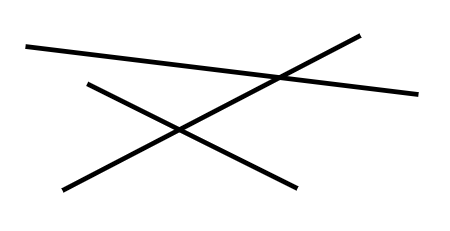
\includegraphics[width=0.4\textwidth]{data/zamiatanie_wariant2_kontrprzyklad.png}
	\caption{ % moze dać podpis to bedzie wiadomo o co chodzi
	 }
	\label{fig:zamiatanie_kontrprzyklad_wariant2}
\end{figure}

\begin{algorithm}[H]
	\caption{(Wariant 2) Znalezienie wszystkich punktów przecięcia w zbiorze odcinków}
	\begin{algorithmic}[1]
		\Procedure{FindIntersectingPoints}{$S$: zbiór odcinków spełniający założenia}
		\State  $X \gets$ \textit{zdarzenia} dla każdego punktu będącego
		krańcem pewnego odcinka z $S$
		\State $Y \gets \emptyset$
		\State $P \gets \text{pusty zbiór punktów}$ 
		\While{$X \not = \emptyset$}
		\State \textit{zdarzenie} = $X.$FindFirst()
		
		\If {\textit{zdarzenie} odpowiada początkowi lub końcowi odcinka}
			\State $s \gets \text{odcinek odpowiadający \textit{zdarzeniu}}$
		\ElsIf{\textit{zdarzenie} odpowiada przecięciu się odcinków}
			\State $s_1, s_2 \gets \text{odcinki odpowiadające \textit{zdarzeniu} (kolejno dolny i górny)}$
		\EndIf
		\State $p \gets \text{punkt odpowiadający \textit{zdarzeniu}}$
		\State
		\If{$p$ jest początkiem odcinika $s$}
		\parIf{$s$ przecina się z $Y$.Above($s$) lub z $Y$.Below($s$)
			oraz
			$x$-owa współrzędna tego przecięcia jest większa niż $x_p$}
		\parState {Dodaj do $X$ \textit{zdarzenie} zawierające $s$, $Y$.Above($s$)
		albo $Y$.below($s$)\footnotemark \, oraz ich punkt przecięcia }
		\EndparIf
		\ElsIf{$p$ jest końcem odcinka $s$}
		\parIf{$Y$.above($s$) przecina się z $Y$.below($s$) oraz $x$-owa współrzędna tego przecięcia jest większa niż $x_p$}
		\parState {Dodaj do $X$ \textit{zdarzenie} zawierające $Y$.Above($s$), $Y$.Below($s$) oraz ich punkt przecięcia }
		\EndparIf
		\Else
		\State $P \gets P \cup \{p\}$
		\State $Y$.Interchange($s_1$, $s_2$)
		\parIf{$s_1$ przecina się z $Y$.Above($s_1$) oraz $x$-owa współrzędna tego przecięcia jest większa niż $x_p$}
		\parState {Dodaj do $X$ \textit{zdarzenie} zawierające $s_1$, $Y$.Above($s_1$) oraz ich punkt przecięcia}
		\EndparIf
		\parIf{$s_2$ przecina się z $Y$.Below($s_2$) oraz $x$-owa współrzędna tego przecięcia jest większa niż $x_p$}
		\parState {Dodaj do $X$ \textit{zdarzenie} zawierające $s_2$, $Y$.Below($s_2$) oraz ich punkt przecięcia}
		\EndparIf
		\EndIf
		\EndWhile
		\State \Return $P$
		\EndProcedure
	\end{algorithmic}
	\label{HasIntersectingSegments2}
\end{algorithm}
\footnotetext{Zawsze będzie to tylko jeden z nich z założenia o braku pionowych odcinków.}

Warto zwrócić uwagę na to, że dodajemy zdarzenie tylko wtedy, kiedy
$x$-owa współrzędna tego przecięcia jest większa niż $x_p$. Gdybyśmy tego nie zrobili,
pojawią się przypadki, w których będziemy badali dwukrotnie ten sam punkt, co 
może sprawiać problemy implementacyjne.

\subsection{Znajdowanie otoczki wypukłej}

\subsubsection{Algorytm Grahama}

W celu opisania algorytmu Grahama potrzebujemy zdefiniować pojęcie lewego oraz prawego skrętu.

\begin{defi}
	Trójkę punktów $(P, Q, R)$ taką, że $(Q-P) \times (R-P) > 0$ nazywamy skrętem w lewo.
\end{defi}
\begin{defi}
	Trójkę punktów $(P, Q, R)$ taką, że $(Q-P) \times (R-P) < 0$ nazywamy skrętem w prawo.
\end{defi}

\begin{minipage}{0.45\linewidth}
	\begin{figure}[H]
		\centering
		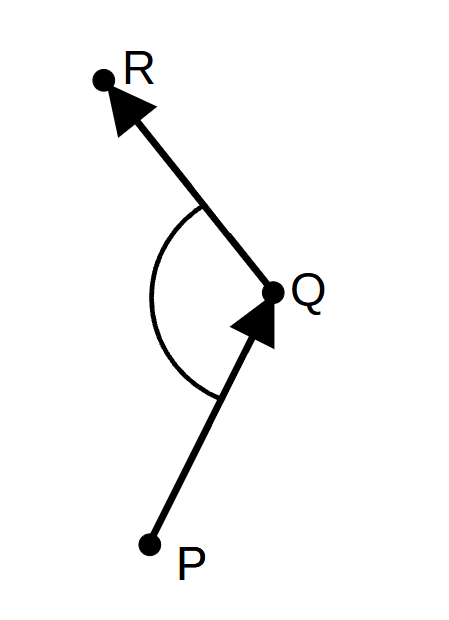
\includegraphics[height=0.45\linewidth]{data/skretwlewo.png}
		\caption{\small Skręt w lewo. Kąt $\angle PQR$ jest wypukły.}
	\end{figure}
\end{minipage}
\hfill
\begin{minipage}{0.45\linewidth}
	\begin{figure}[H]
		\centering
		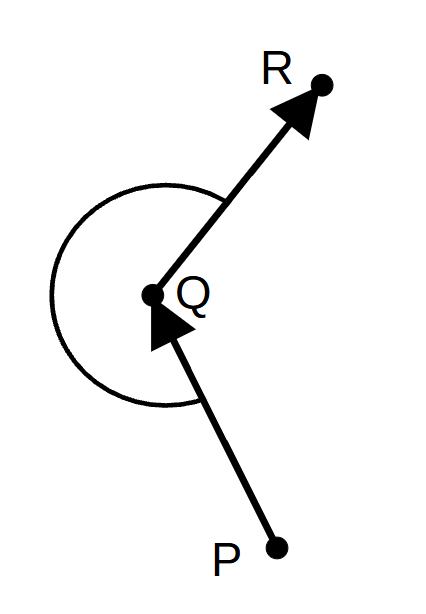
\includegraphics[height=0.45\linewidth]{data/skretwprawo.png}
		\caption{\small Skręt w prawo. Kąt $\angle PQR$ jest wklęsły.}	
	\end{figure}
\end{minipage}

\begin{algorithm}[H]
	\caption{Algorytm Grahama znajdowania otoczki wypukłej}\label{alg:graham}
	\begin{algorithmic}[1]
		\Procedure{SortPoints}{$P$: zbiór punktów}
			\State $P[0] \gets $ punkt z $P$ o najmniejszej współrzędnej $y$ (w przypadku równości $y$ ten o najmniejszej współrzędnej $x$)
			\State $P[1 \dots n-1] \gets $ pozostałe punkty posortowane według wzrastających kątów, jakie tworzą odcinki o początku w $P[0]$ i końcu w $P[k]$ z osią $X$ (w przypadku równości kątów, rozważamy tylko punkt skrajny)
		\EndProcedure
		\Procedure{Graham}{$P$: zbiór punktów}
			\State $P \gets \textsc{SortPoints}(P)$
			\State $S \gets \text{stos}()$
			\State $S$.Push($P[0]$)
			\State $S$.Push($P[1]$)
			\For {$k = 2,3, \dots, n-1$}
				\While{($S$.BelowTop(), $S$.Top(), $P[k]$) nie jest skrętem w lewo}
					\State $S$.Pop()
				\EndWhile
				\State $S$.Push($P[k]$)
			\EndFor
			\State \Return $S$
		\EndProcedure
	\end{algorithmic}
\end{algorithm}

\begin{fact}[Opis wielokąta wypukłego]
	\label{fact:wielwypukly}
	Niech $W$ będzie wielokątem reprezentowanym przez ciąg punktów. Wielokąt nie ma samoprzecięć i każda kolejna (modulo $|W|$) trójka punktów w $W$\! tworzy skręt w lewo wtedy i tylko wtedy, gdy $W$ jest wielokątem wypukłym.
\end{fact}

\begin{theorem}[Poprawność algorytmu Grahama]
	Algorytm Grahama poprawnie znajduje otoczkę wypukłą danego zbioru punktów.
	\begin{proof}
		Niech $P$ to pewien zbiór punktów, wtedy przez $\operatorname{CH}(P)$, będziemy rozumieli otoczkę wypukłą na zbiorze punktów $P$.
		\phantom{a}
		\begin{enumerate}
			\item Pokażemy, że $P[0]$ jest wierzchołkiem otoczki wypukłej $P$. 
			
			Załóżmy nie wprost, że $P[0]$ nie jest wierzchołkiem $\operatorname{CH}(P)$. Wtedy istnieje krawędź $\operatorname{CH}(P)$ znajdująca się pod $P[0]$, co oznacza, że istnieje punkt (koniec tej krawędzi) o mniejszej współrzędnej $y$ -- sprzeczność, bo z definicji $P[0]$ jest punktem o najmniejszej współrzędnej $y$.
			
			Analogicznie dowodzimy w przypadku, gdy jest kilka punktów o tej samej współrzędnej $y$.
		
			\item Jako $S_k$ oznaczmy ciąg punktów na stosie po dodaniu punktu $P[k]$ do otoczki (tzn. po $(k-1)$-szej iteracji). Pokażemy niezmiennik pętli \textit{for}: punkty w $S_{k}$ stanowią otoczkę wypukłą zbioru $\{P[0], P[1], \dots, P[k]\}$.
			
			\begin{itemize}
				\item Baza indukcji. Przed pętlą \textit{for} ciąg $S_1$ opisuje odcinek $(P[0], P[1])$, który naturalnie jest otoczką wypukłą zbioru  $\{P[0], P[1]\}$.
				
				\item Krok indukcyjny. Zakładamy, że dla każdego $k'$, $k'<k$ w $k'$-tej iteracji $S_{k'}$ jest otoczką wypukłą zbioru $\{P[0], P[1], \dots P[k']\}$. 
				Chcemy pokazać, że $S_k$ opisuje wielokąt wypukły, który jest otoczką zbioru $P$.
				
				\begin{enumerate}				
					\item Po zakończeniu pętli \textit{while}, $S$.BelowTop(), $S$.Top() i $P[k]$ tworzą skręt w lewo (z warunku pętli). Również dowolne 3 kolejne elementy $S$ tworzą skręt w lewo ($S$ jest podciągiem $S_{k-1}$, w którym zachodzi to z założenia indukcyjnego oraz faktu \ref{fact:wielwypukly}). Oznacza to, że dowolne 3 kolejne elementy z $S_k = S \cup \{P[k]\}$ tworzą skręt w lewo. 
					
					\item Ponadto tablica $P$ jest posortowana według rosnących kątów, więc $P[k]$ znajduje się na lewo od prostej przechodzącej przez punkty $P[0]$ oraz $S$.Top() (rysunek \ref{fig:graham:samoprzeciecie}). Nie powstanie zatem samoprzecięcie.
					
					\begin{minipage}{0.47\linewidth}
						\begin{figure}[H]
							\centering
							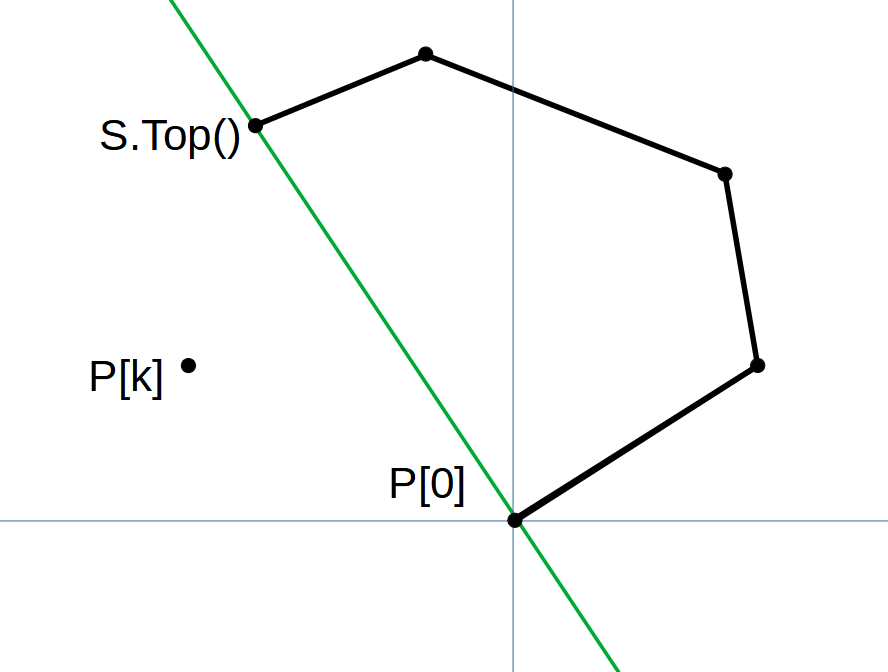
\includegraphics[width=\textwidth]{data/graham1.png}
							\caption{\small Samoprzecięcie mogłoby powstać, gdyby dodawany punkt był na prawo od zielonej prostej.}
							\label{fig:graham:samoprzeciecie}
						\end{figure}
					\end{minipage}
					\hfill
					\begin{minipage}{0.47\linewidth}
						\begin{figure}[H]
							\centering
							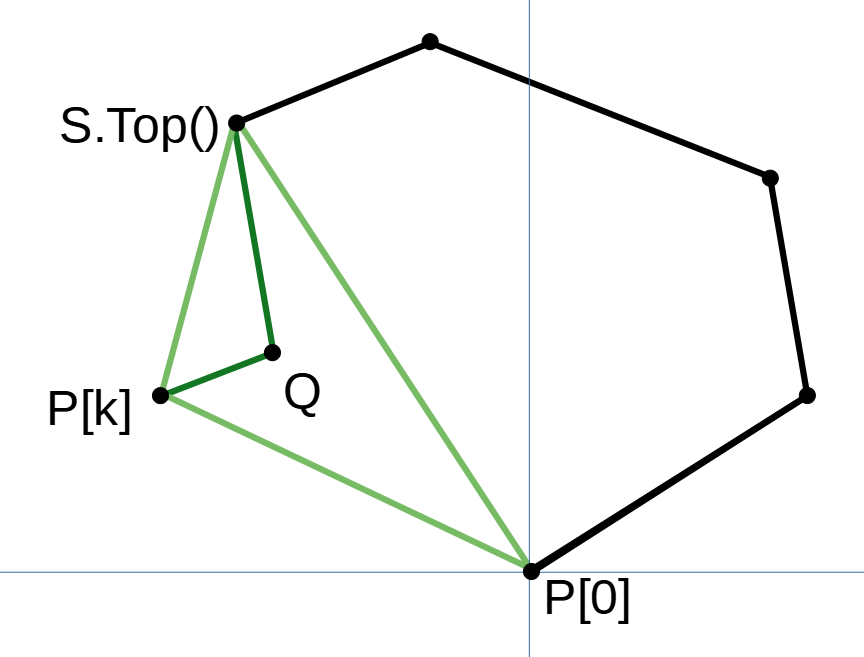
\includegraphics[width=\textwidth]{data/graham2.png}
							\caption{\small Usuwając punkty z $S$ w pętli \textit{while} mamy pewność, że nie leżą one na brzegu szukanej otoczki wypukłej}
							\label{fig:graham:usuwanie}
						\end{figure}
					\end{minipage}				

					\item Niech $\bar{S}$ będzie zbiorem punktów zdjętych w ostatnim wykonaniu pętli \textit{while} ze stosu $S_{k-1}$.
					Weźmy dowolny $Q \in \bar{S}$. Z prawoskrętności trójki ($S$.Top(), $Q$, $P[k]$) wynika, że kąt wyznaczony przez tę trójkę jest wklęsły, zatem $Q$ leży we wnętrzu trójkąta $(P[k], P[0], S.\operatorname{Top}())$ (rysunek \ref{fig:graham:usuwanie}). Oznacza to, że zbiór $\bar{S}$
					 znajduje się wewnątrz wielokąta wypukłego $S_k$. Z założenia indukcyjnego wszystkie punkty z $\{P[0], \dots, P[k-1]\}$ leżą wewnątrz wielokąta wypukłego opisanego przez $S_{k-1}$.
					 Skoro wszystkie punkty z $S_{k-1}$ należą albo do $S_k$
					 albo leżą wewnątrz wielokąta wypukłego $S_k$, to $S_k$ musi stanowić otoczkę zbioru $\{P[0], \dots, P[k]\}$.
					 
				\end{enumerate}	
				Punkty (a) oraz (b) faktu 1. implikują, że $S_k$ jest wielokątem wypukłym, natomiast (c), że wielokąt wypukły $S_k$ stanowi otoczkę wypukłą
				zbioru \linebreak $\{P[0], P[1], \ldots, P[k]\}$, co oznacza, że niezmiennik 
				jest prawdziwy.			
			\end{itemize}
			
			
			\item Na stosie $S$ znajdują się punkty $P[0]$ oraz $P[1]$, w każdym
			momencie wykonywania się algorytmu.
			
			Niech $P_k := \{P[0], P[1], \ldots, P[k]\}$.
			
			\begin{enumerate}
				\item Pokażmy, że $P[0]$ jest wierzchołkiem $\operatorname{CH}(P_k)$ dla każdego $k \in \{0, 1, \ldots n\}$.
				
				Załóżmy nie wprost, że $P[0]$ nie jest wierzchołkiem $\operatorname{CH}(P_k)$ dla pewnego 
				$k \in \{0, 1, \ldots n\}$. Wtedy istnieje krawędź
				w $\operatorname{CH}(P_k)$ znajdująca się pod $P[0]$, co oznacza, że istnieje punkt (koniec tej krawędzi) o mniejszej współrzędnej $y$ -- sprzeczność, bo z definicji $P[0]$ jest punktem o najmniejszej współrzędnej $y$. Analogicznie dowodzimy w przypadku, gdy jest kilka punktów o tej samej współrzędnej $y$. 
				
				\item Pokażmy, że $P[1]$ jest wierzchołkiem $\operatorname{CH}(P_k)$ dla każdego $k \in \{0, 1, \ldots n\}$.
				
				Z posortowania wierzchołków $P_k$ wynika, że pod prostą przechodzącą przez punkty $P[0]$ i $P[1]$ nie może istnieć 
				żaden inny punkt należący do $P_k$. Oznacza to, że nie istnieje punkt $P[i]$, gdzie $i \in \{0, 1, \ldots k\}$, taki, że 
				trójka ($P[0]$, $P[1]$, $P[i]$) jest skrętem w prawo. Z tego faktu implikujemy, że $P[1]$ również należy do $\operatorname{CH}(P_k)$.
				
			\end{enumerate}
			Skoro $P[0], P[1] \in \operatorname{CH}(P_k)$ to z 1., wiadomo, że $P[0], P[1] \in S_k$ dla każdego $k \in \{0, 1, \ldots n\}$.
			
		\end{enumerate}
		
		Fakt 2., mówi, że zawsze jesteśmy wstanie dokonać sprawdzenia 
		skrętu trójki ($S$.BelowTop(), $S$.Top(), $P[k]$), gdzie $k \in
		\{1, 2, \ldots, n\}$.
		
		Z faktu 1., po $n-1$ iteracjach pętli \textit{for} ciąg punktów $S$ opisuje otoczkę wypukłą wszystkich punktów z $P$. 
	\end{proof}
\end{theorem}

